\chapter{Sekwencjonowanie i adnotacja genomu}
\label{section:sekwencjonowanie_i_adnotacja}

\subsection*{Centralny dogmat bioinformatyki}
Podstawowym założeniem w bioinformatyce jest następująca zależność:
Informacja, która jest zawarta w sekwencji nukleotydowej przekłada się na strukturę przestrzenną białek i innych cząsteczek, które są w genomie zakodowane. 
Dzięki odpowiednio uformowanej strukturze przestrzennej, białka stają się aktywne i mogą oddziaływać w przestrzeni komórkowej, pełniąc różne funkcje molekularne i angażując się w procesy biochemiczne. 
Funkcją biochemiczną może być np. reakcja w którą wchodzi dane białko łącząc się z inną substancją. 
Efekt końcowy oddziaływań zbioru wybranych białek obserwujemy w postaci np. wyglądu zewnętrznego (fenotypu), zachowania lub funkcjonowania organizmu.

Informacje sekwencyjne jesteśmy w stanie eksperymentalnie pozyskać bardzo łatwo. Trudniej jest określić struktury przestrzenne i funkcje biochemiczne jakie pełnią.
Obecnie nacisk jest wywierany na ustalenie procesu w jaki sposób na podstawie sekwencji możemy określić strukturę przestrzenną bądź później, funkcję danego związku chemicznego.
Z samej obserwacji fenotypu nic nie wynosimy. Dążymy do tego aby dowiedzieć się jakie konkretne białka odpowiadają za dany fenotyp. Chcemy posiąść kompletną wiedzę na temat funkcjonowania organizmu. Kryje się za tym znajomość wszystkich genów jakie mogą w tym organiźmie występować, odmian, mutacji i ch wzajemnych wpływów.

\begin{figure}[h]
	\centering
	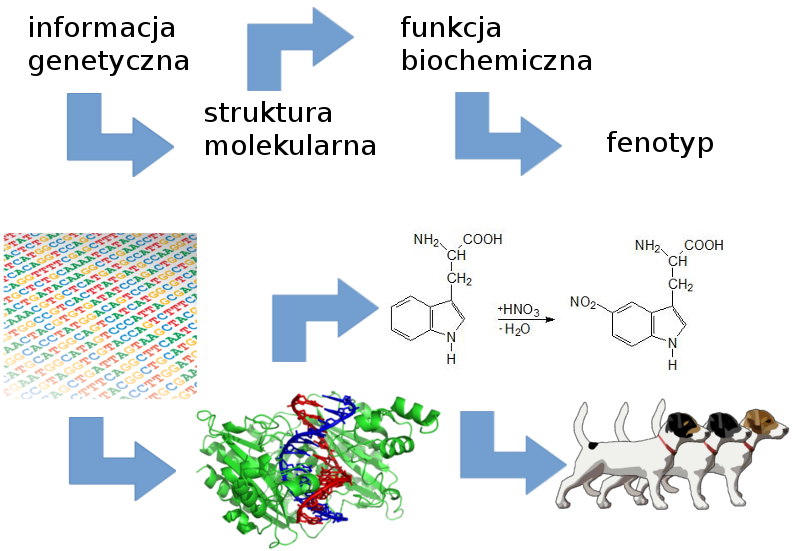
\includegraphics[width=0.9\textwidth]{img/centralny-dogmat.png}
	\caption{Centralny dogmat bioinformatyki}
	\vspace{-0.5cm}
	\caption*{\scriptsize Źródła: 
		\url{http://www.wikiwand.com/en/DNA},
		\url{http://igoscience.com/dna-sequence-genetic-code/} \\
		\url{https://commons.wikimedia.org/wiki/File\%3AReakcja\_ksantoproteinowa\_dla\_tryptofanu.jpg}, \\
		\url{https://www.russell-terrier.org/index.php/blog/56-maść-jrt-i-prt-w-praktyce-część-vi-fenotyp}
	}
	\label{img:centralny-dogmat}
\end{figure}

\subsection*{Problemy bioinformatyki}
Bioinformatyka, jak każda dziedzina naukowa boryka się z pewnymi problemami. 
Problem dotyczący baz danych polega na tym, że wiele baz powstaje jako wynik grantu badawczego a potem z tymi danymi często nic się nie dzieje.

Każdego dnia ludzkość poznaje tysiące nowych sekwencji, które są deponowane w cyfrowych przechowalniach. 
,,Podstawowe bazy'' są tworzone i z powodzeniem wykorzystywane do naukowych doświadczeń. W oparciu o nie powstają "bazy wtórne", bazujące na wynikach z wcześniejszych, podstawowych eksperymentów. 
Bazy wtórne gromadzą najczęściej zbiór informacji pochodzący z różnych źródeł.
Niejednokrotnie zdarza się, że do bazy pierwotnej są wprowadzane modyfikacje, które nie zostają już uwzględnione w późniejszych bazach wtórnych. 
Błędy te propagują się na następne projekty. 
Opisany problem dotyczy oczywiście również projektów bioinformatycznych, szczególnie w sytuacjach braku możliwości ich kontynuacji lub weryfikacji.
Jest to jeden z poważniejszych problemów z jakim obecnie boryka się świat bioinformatyki.

Wspomniane zbiory danych często są ogromne. 
Sekwencja przykładowego genomu człowieka zajmuje ponad 3GB, natomiast opis samego eksperymentu sekwencjonowania może zająć nawet kilkaset gigabajtów. 
Pojawiający się problem jest natury technicznej - chodzi o sposób przechowywania danych.
Okazuje się, że często bardziej opłaca się laboratorium ponownie przeprowadzić eksperyment sekwencjonowania, niż przechowywać wyniki doświadczeń na dyskach, gdyż jest to zbyt kosztowne.

Kolejnym problemem jest mnogość standardów. 
Często gdy jest jakiś problem, rozwiązanie projektowane jest od podstaw. 
Takie podejście skutkuje tym, że dla pojedynczego zadania, mamy kilkanaście bądź kilkadziesiąt różnych metod, które nie koniecznie są ze sobą kompatybilne. 
Jednym z głównych problemów, z jakim zmagają się biolodzy przy analizie danych jest to, że wyjście z jednego programu nie jest kompatybilne z wejściem drugiego programu, który potrzebują aktualnie wykorzystać. 
Próby rozwiązania takiego kłopotu skutkują często zdefiniowaniem kolejnego standardu, co może jeszcze bardziej skomplikować sytuację jeśli nowy sposób się nie zostanie przyjęty przez większe grono naukowców.

%-niekontynuowane projekty \\
%-dane bazują na eksperymentach, błędy propagujące się \\
%-wiele różnych standardów, niekompatybilne \\
%-nieinformatyczni biolodzy \\
%-sposoby finansowania nauki \\

\section{Sekwencjonowanie i asembling DNA}
Sekwencjonowanie to jedna z technik biologii molekularnej, pozwalająca na odczytanie kolejności nukleotydów w cząsteczce DNA.

Najlepiej byłoby, gdyby projekt genomu reprezentował kompletną sekwencję nukleotydową wszystkich chromosomów danego gatunku. 
Jednak w rzeczywistości, istnieje wiele potencjalnych problemów związanych z procesem sekwencjonowania. Nie istnieje bowiem, jedna, prawdziwa sekwencja dla gatunku z powodu indywidualnej zmienności genetycznej jednostek. 
Nawet komórki tego samego osobnika mogą różnić się w zawartości genetycznej z powodu mutacji somatycznych. Złożony genom będzie tylko jedną reprezentacją wariacji występującej u danego gatunku. 
Zasadniczo sekwencjonuje się tylko jednego osobnika, ale czasami genom stanowi konsensus wielu połączonych próbek (projekt HUGO). 
Należy zdawać sobie sprawę, że procesowi sekwencjonowania zawsze będą towarzyszyć błędy na poziomie poszczególnych nukleotydów oraz ich kolejności (błędy montażu). 
Każdy złożony genom jest wynikiem serii złożeń metodami heurystycznymi i powinien być traktowany jako robocza hipoteza.

\begin{figure}[h]
	\centering
	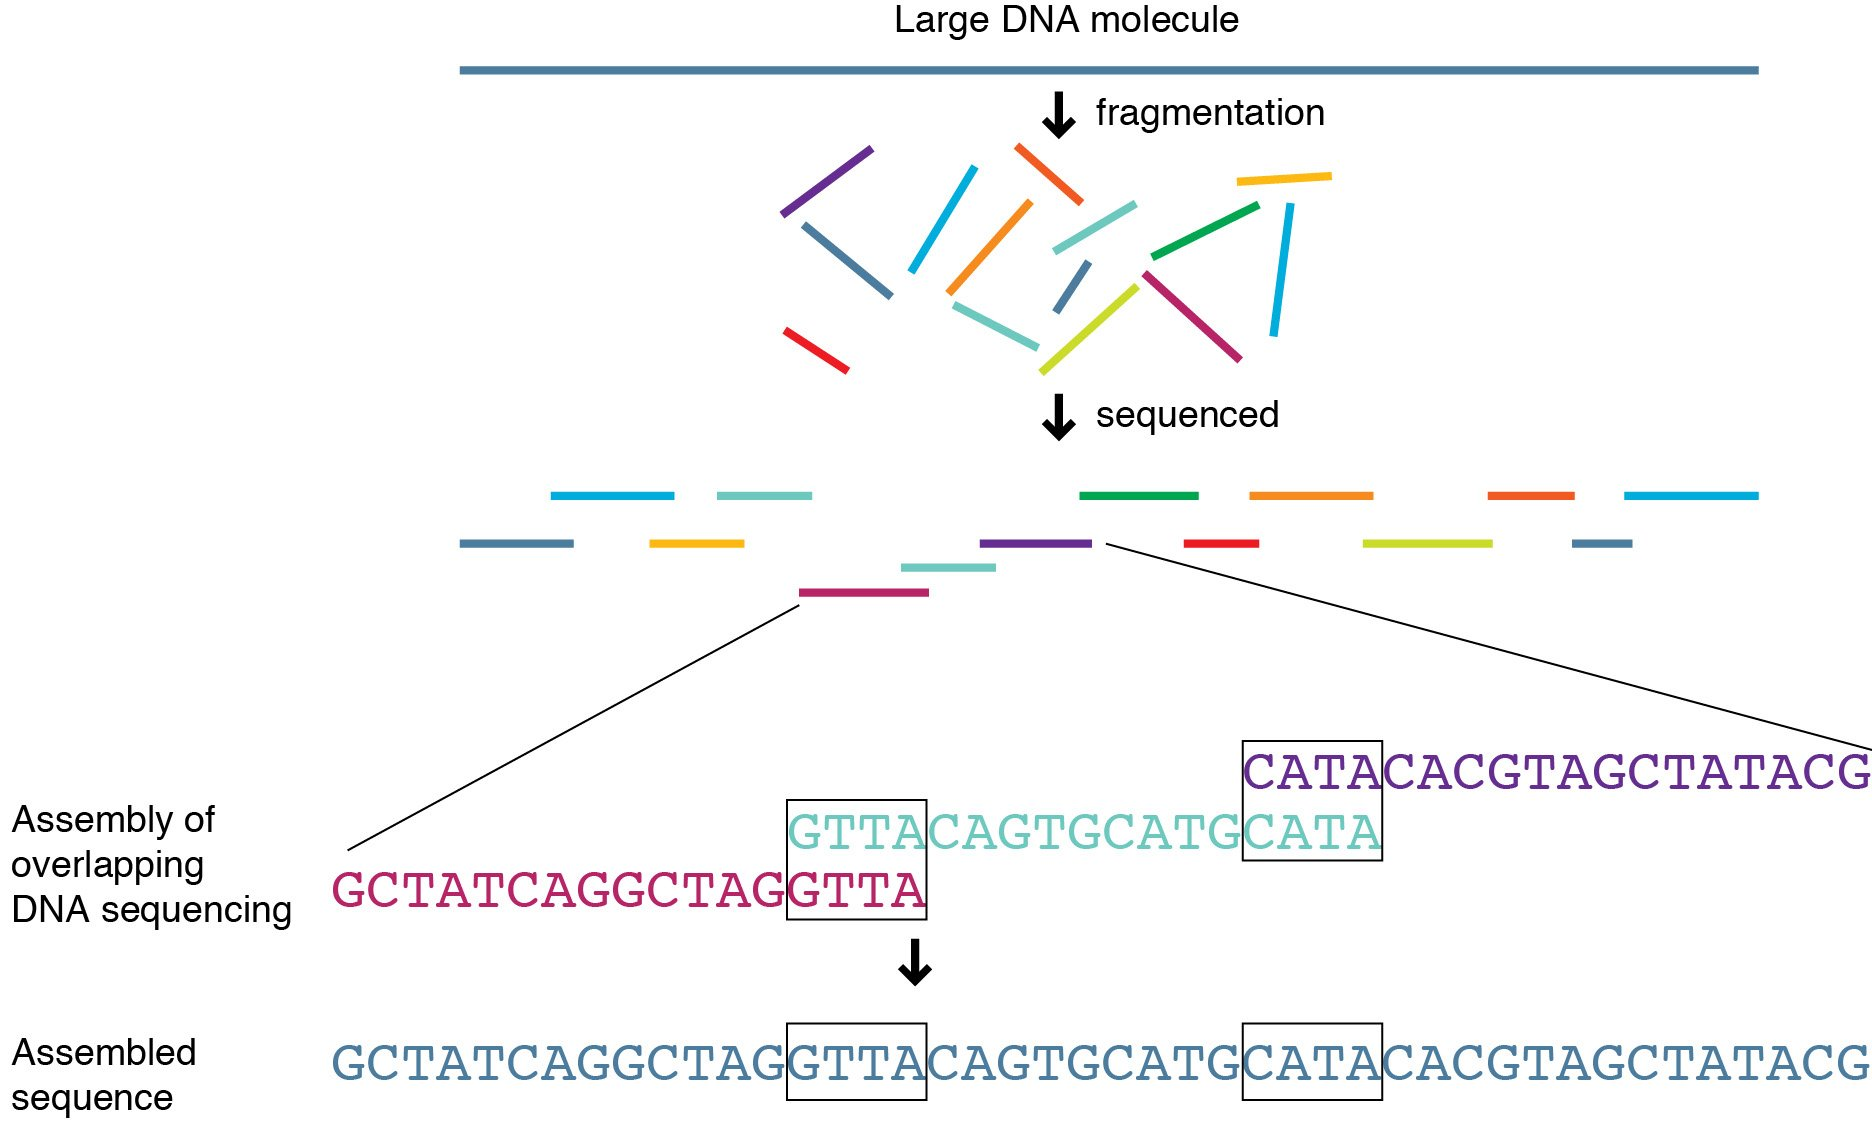
\includegraphics[width=0.9\textwidth]{img/sequenctioning-process.png}
	%zdjecie z %http://knowgenetics.org/whole-genome-sequencing/
	\caption{Schemat sekwencjonowania}
	\vspace{-0.5cm}
	\caption*{\scriptsize Źródło: \url{http://knowgenetics.org/whole-genome-sequencing/}}
	\label{img:schemat-sekwencjonowania}
\end{figure}

Większość projektów, w początkowej fazie sekwencjonowania kieruje się strategią polegającą na losowym pocięciu DNA na bardzo małe fragmenty.
W zależności od wykorzystanej technologii, fragmenty mogą mieć różne długości. Istnieje trend w kierunku przeprowadzania odczytów technikami dającymi coraz krótsze fragmenty. 
Tradycyjne sposoby (Sanger) dawały fragmenty długości około 1000 par zasad. Obecnie wykorzystywane techniki dające najkrótsze rezultaty osiągają wyniki rzędu dziesiątek pz. (SOLiD, Illumina - rys.\ref{img:sekwencjoner-illumina}).

\begin{figure}[h]
	\centering
	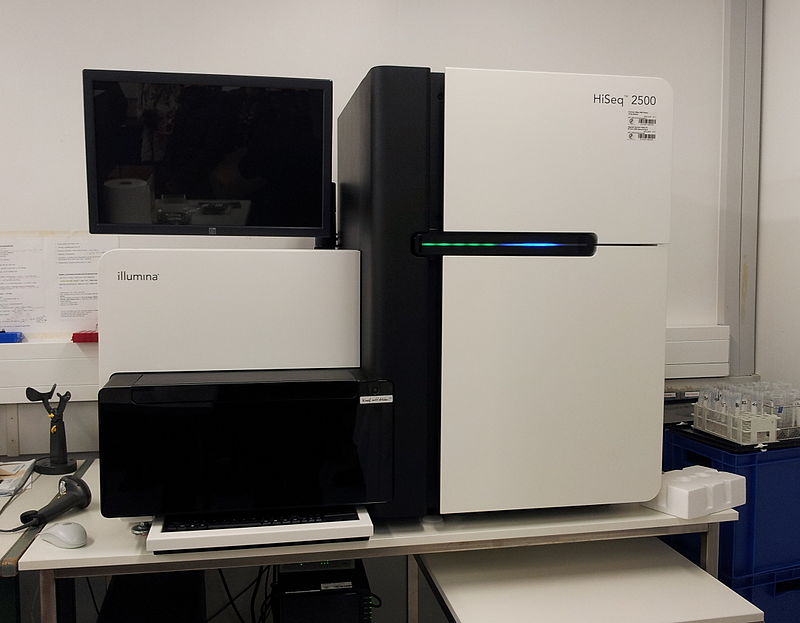
\includegraphics[width=0.75\textwidth]{img/sekwencjoner-illumina.jpg}
	%zdjecie z http://wiedza.alkahest.umcs.pl/jak-limfocyty-t-przekazuja-informacje/
	\caption{Sekwencjoner Illumina HiSeq 2500}
	\vspace{-0.5cm}
	\caption*{\scriptsize Źródło: \url{http://wiedza.alkahest.umcs.pl/jak-limfocyty-t-przekazuja-informacje/}}
	\label{img:sekwencjoner-illumina}
\end{figure}

Następie, w procesie asemblingu, fragmenty sekwencji są składane w dłuższe odcinki. Dobór algorytmu jest zależny od długości odcinków zsekwencjonowanych w poprzednim etapie. Jest to proces skomplikowany i wykorzystywane są do tego zasobożerne programy. 
Efektem początkowego składania sekwencji są kontigi.
Na dalszych etapach, po analizach wykorzystujących biblioteki dłużych sekwencji DNA, kontigi są zespalane w struktury zwane skafoldami.
Mają one zazwyczaj postać sekwencji z lukami o znanej długości - dziury oznaczane są znakiem ,,N''.

\section{Adnotacje}
Aby wykorzystać cały potencjał sekwencji genomu, musi on zostać opatrzony adnotacjami, które zawierają istotne informacje z biologicznego punktu widzenia. Kompletna adnotacja genomu stanowi duże wyzwanie dla biologów, a jej wyniki są w dużej mierze uzależnione od jakości złożenia genomu w procesie asemblingu.

Adnotacja genomu jest procesem odnalezienia regionów kodujących, zidentyfikowania genów oraz określenia funkcji jakie pełnią. Adnotacją możemy nazywać np. przypis będący notatką dodaną jako wyjaśnienie bądź komentarz. Dzielą się na przypisy:
\itemize{
	\item strukturalne (identyfikacja obiektów genomowych)
	\item funkcjonalne (biologiczne informacje związane z obiektami genomowymi)
}
\\
Proces adnotacji można podzielić na 3 główne fazy:
\enumerate{
	\item Identyfikacja niekodujących fragmentów.
	\item Przewidywanie genów.
	\item Dołączenie biologicznych informacji.
}\\

Większość technik wykorzystuje narzędzia oparte o wyszukiwanie homologicznych sekwencji używając do tego celu publiczne bazy danych genomów. Przewidywanie genów to czynność mająca na celu zidentyfikowanie fragmentów DNA, które odpowiedzialne są za kodowanie białek. Wśród organizmów zbudowanych z komórek posiadających jądro komórkowe z chromosomami (eukarioty), odcinki kodujące sekwencję aminokwasów nazywane są eksonami, które zazyczaj oddzielone są fragmentami niekodującymi - intronami (rys.\ref{img:intron-exon}).

\begin{figure}[h]
	\centering
	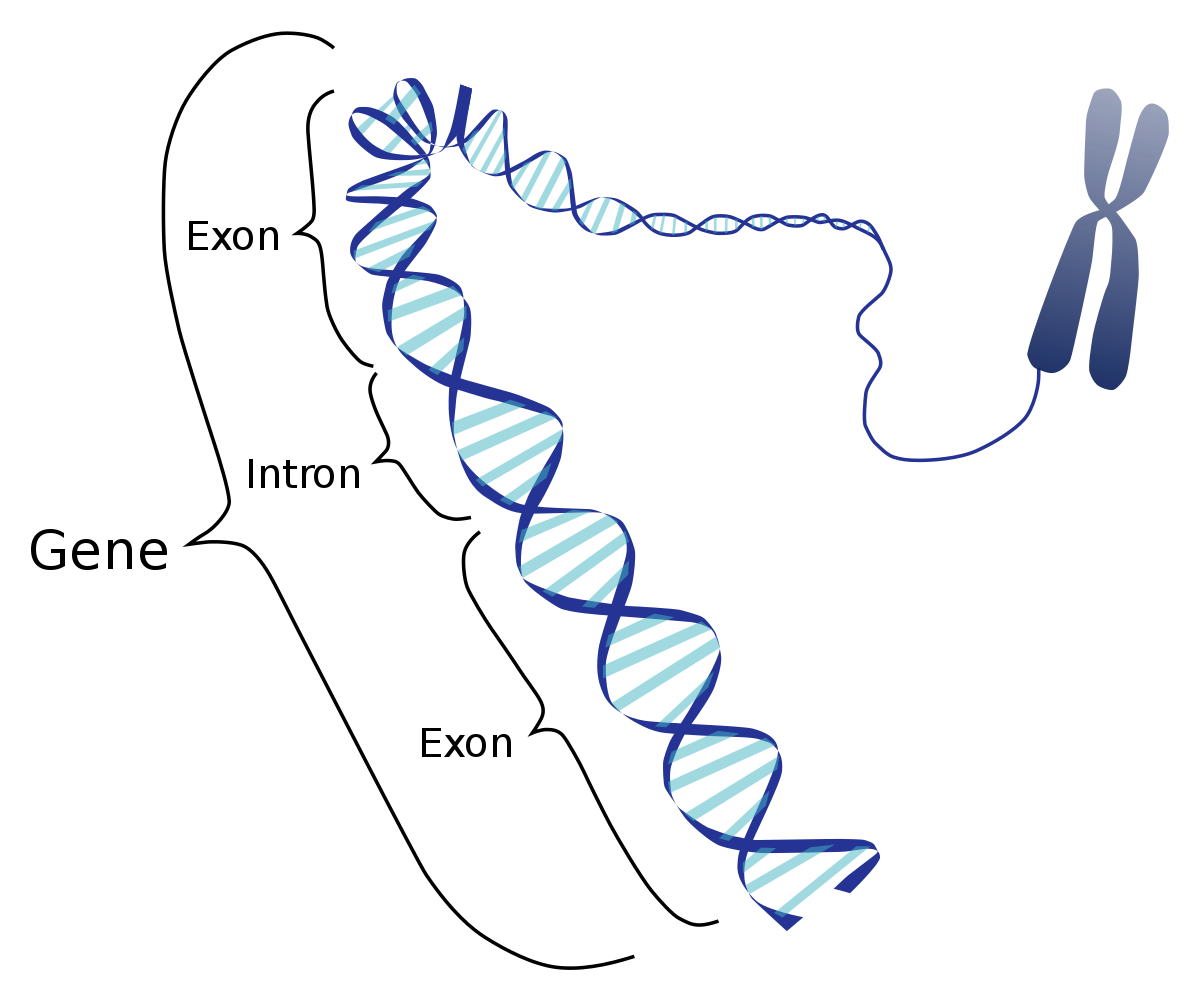
\includegraphics[width=0.75\textwidth]{img/intron-exon.png}
	\caption{Reprezentacja intronów i eksonów z genem zawierającym pojedynczy intron i dwa eksony.}
	\vspace{-0.5cm}
	\caption*{\scriptsize Źródło: \url{https://en.wikipedia.org/wiki/File:Gene\_Intron\_Exon\_nb.svg}}
	\label{img:intron-exon}
\end{figure}


\section{Prezentacja danych}
Kolejnym etapem projektu poznania genomu jest zazwyczaj umieszczenie go w przeglądarce genomów wraz z adnotacjami. Są to programy mające wygodny interfejs graficzny, gromadzące i w przystępny sposób prezentujące informacje uzyskane w poprzednich etapach badań. Dzięki nim naukowcy mają możliwość przede wszystkim łatwego dostęp do danych, a także posiadają wygodne narzędzie do dalszych prac. 
Ważnym aspektem jest fakt, że dzięki przeglądarkom mogą dzielić się wynikami prac z innymi zespołami badawczymi, bez czego postęp biotechnologiczny rozwijałby się znacznie wolniej.

Dane wizualizowane są najczęściej w sposób interaktywny pozwalając na obserwację genomu z perspektyw makro (chromosomów) i mikro (poszczególne geny, ciągi nukleotydowe).

Udostępnienie genomu umożliwia rozpoczęcie wielu prac z zakresu jego szczegółowej analizy, poczynając od analizy struktury i funkcji genów a kończąc na analizach filogenetycznych obejmujących całe genomy. 
Celem analiz filogenetycznych jest rekonstrukcja historii ewolucji  organizmów. W klasycznym podejściu historia ewolucji jest odtwarzana na podstawie porównań cech morfologicznych i fizjologicznych badanych organizmów.
Filogenetyka molekularna rekonstruuje związki filogenetyczne między badanymi sekwencjami, opierając się na założeniu, iż sekwencje przodka mutują w sekwencje potomków a podobne gatunki są genetycznie blisko spokrewnione.
Powszechnym przykładem wykorzystania udostępnionego genomu jest analiza sekwencji, na której badacz projektuje inne sekwencje np. startery do PCR, czy startery do RT-PCR\footnote{metoda stosowana do ilościowego określania ekspresji specyficznych genów, również w diagnostyce medycznej i mikrobiologicznej.}.


\section{Przegląd literatury - istniejące rozwiązania}

\subsection*{Najpopularniejsze przeglądarki}
\begin{itemize}
	% https://en.wikipedia.org/wiki/UCSC_Genome_Browser
	% http://genome.ucsc.edu/
	\item \href{https://genome.ucsc.edu}{\emph{UCSC browser}} (rys.\ref{img:przegladarka-UCSC}) \label{przegladarka-UCSC}
	
	przeglądarka on-line, opracowana na Uniwersytecie Kalifornijskim w~Santa Cruz w 2000 roku; główni autorzy - Jim Kent, David Haussler; zaimplementowana w~większości w~języku~C. Udostępniana darmowo dla akademickich zastosowań, dla komercyjnych wymagana licencja \emph{Kent Informatics}. Zawiera 46 gatunków organizmów. Pozwala wyświetlać sekwencje o dowolnym rozmiarze - od pojedynczych zasad po chromosomy. Badacze mogą wyświetlać własne dane i wyświetlać je w kontekście referencyjnego genomu. Widoki tworzone przez użytkowników mogą być udostępniane innym użytkownikom.
	
	W porównaniu do CuGene:
	brak funkcjonalności widoków z priorytetyzacją nakładających się na siebie typów danych. Brak algorytmów wyszukiwania Knutha-Morrisa-Pratta i Smitha-Watermana. Skomplikowane narzędzie, trudne dla początkujących użytkowników.
	\begin{figure}[h]
		% https://en.wikipedia.org/wiki/UCSC_Genome_Browser#/media/File:BrowserFoxp2.jpg
		\centering
		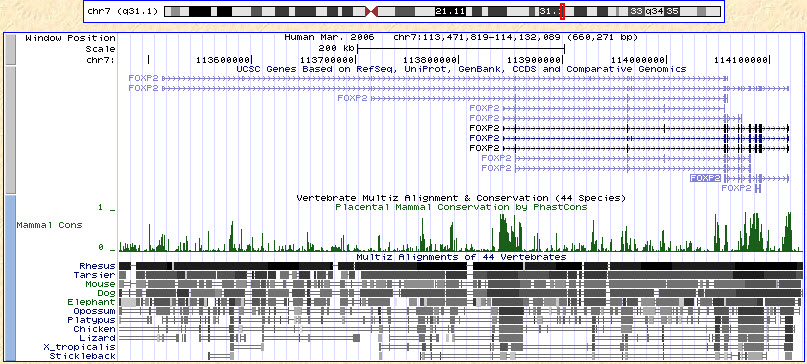
\includegraphics[width=0.75\textwidth]{img/browser-UCSC.jpg}
		\caption{Przeglądarka UCSC.}
		\vspace{-0.5cm}
		\caption*{\scriptsize Źródło: \url{https://en.wikipedia.org/wiki/UCSC\_Genome\_Browser\#/media/File:BrowserFoxp2.jpg}}
		\label{img:przegladarka-UCSC}
	\end{figure}
	
%%%%%%%%%%%%%%%%%%
	\item \href{http://gbrowse.org}{\emph{Gbrowse}} (rys.\ref{img:przegladarka-gbrowse})
	\label{przegladarka-Gbrowse}
	% http://gmod.org/wiki/GBrowse
	
	projekt napisany w Pearlu, przeglądarka on-line; powstała w 2002 roku; funkcjonuje na licencjach \textit{GPL 2.0} oraz \textit{Artistic Licence 2.0}; wielojęzykowa; aktywnie wspierana i wykorzystywana, jedna z najpopularniejszych, aczkolwiek w czasie pisania pracy, główna strona projektu (\textit{http://gbrowse.org/}) była nieosiągalna. Pozwala m.in. na tworzenie linków do dowolnych adnotacji, nawigację poprzez przewijanie, przybliżanie, wspiera format danych GFF, zapamiętuje ustawienia użytkownika podczas trwania sesji. Łączy się z różnymi publicznymi bazami danych (\textit{BioSQL}, \textit{Chado}) Na tle innych przeglądarek wyróżnia się architekturą umożliwiającą wykorzystanie edytowalnych pluginów firm trzecich.
	\begin{figure}[h]
		% http://gmod.org/mediawiki/images/1/10/GBrowse_screenshot1.png
		\centering
		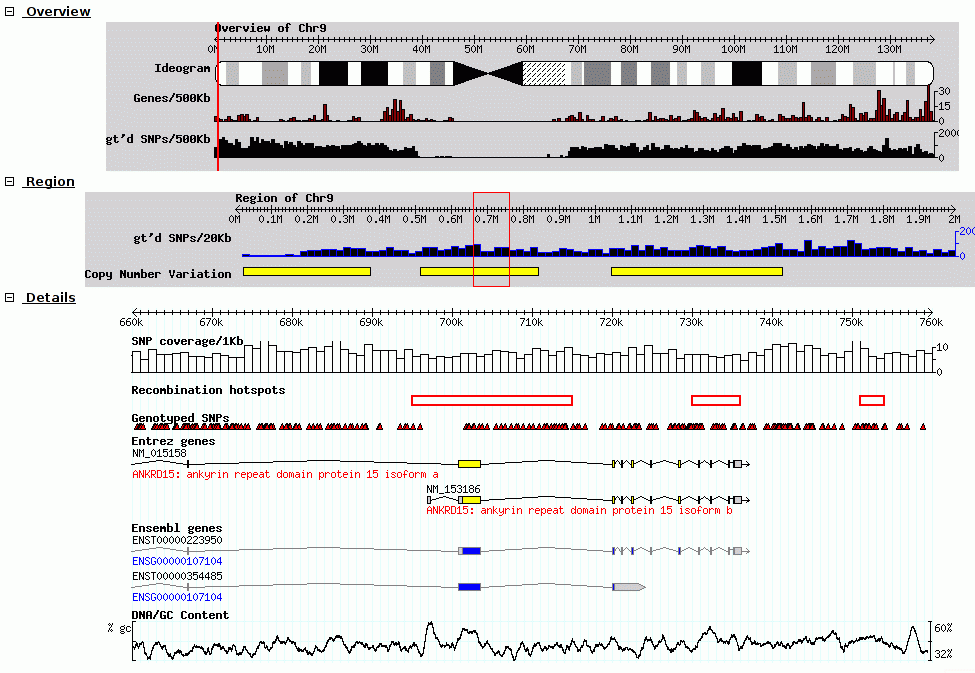
\includegraphics[width=0.75\textwidth]{img/browser-gbrowse.png}
		\caption{Przeglądarka GBrowse.}
		\vspace{-0.5cm}
		\caption*{\scriptsize Źródło: \url{http://gmod.org/mediawiki/images/1/10/GBrowse\_screenshot1.png}}
		\label{img:przegladarka-gbrowse}
	\end{figure}
	
	W porównaniu do CuGene:
	brak funkcjonalności widoków z priorytetyzacją nakładających się na siebie typów danych. Brak algorytmów wyszukiwania Knutha-Morrisa-Pratta i Smitha-Watermana.	
	\\
	
%%%%%%%%%%%%%%%%
	\item \href{http://www.ensembl.org}{\emph{ENSEMBL}} \label{przegladarka-ENSEMBL} (rys.\ref{img:przegladarka-ensembl})
	% http://www.ensembl.info/about/
	% https://en.wikipedia.org/wiki/European_Bioinformatics_Institute
	
	projekt rozpoczęty w celu opisania genomu człowieka i~udostępnienia go w sieci w 1999 roku. Powstał we współpracy pomiędzy EMBL-EBI\footnote{EBI (ang. European Bioinformatics Institute), jest częścią EMBL (ang. European Molecular Biology Laboratory)} a WSI\footnote{WSI (ang. Wellcome Sanger Institute)}. W projekcie uczestniczy 8 zespołów - łącznie około 50 członków. Udostępnione genomy są w większości takie jak w przelgądarce UCSC. Udostępnia API pozwalające pisać samodzielnie skrypty do pozyskiwania interesujących porcji danych.
	
	Zasadniczą różnicą w porównaniu do CuGene jest struktura bazy danych. W projekcie ENSEMBL zastosowano klasyczne podejście polegające na zaprojektowaniu bazy w formie niegenerycznej, odzwierciedlającej biologiczne obiekty w naturze. Na diagramie bazodanowym (rys.\ref{img:db-ensebl}) widać takie tabele jak markery, eksony, transkryptomy, allele, geny itd.
	%https://www.ensembl.org/info/docs/api/core/features_analyses_core.pdf
	
	\begin{figure}[h]
		% https://en.wikipedia.org/wiki/File:Ensembl_release58_sgcb_screenshot.png
		\centering
		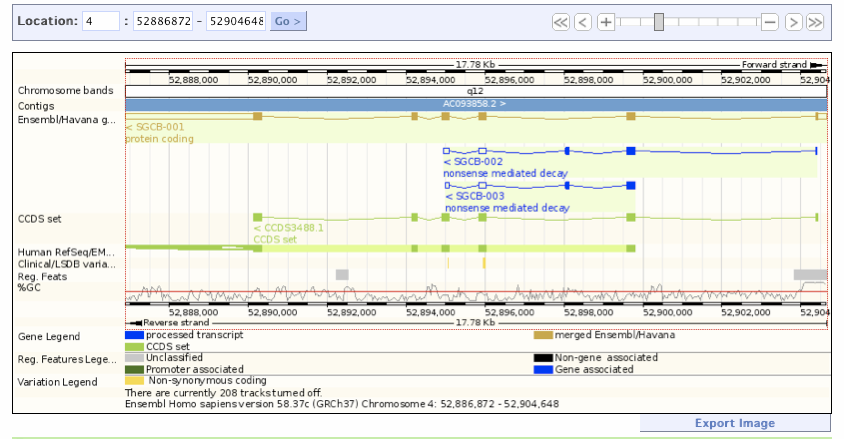
\includegraphics[width=0.75\textwidth]{img/browser-ensembl.png}
		\caption{Przeglądarka EMSEMBL.}
		\vspace{-0.5cm}
		\caption*{\scriptsize Źródło: \url{https://en.wikipedia.org/wiki/File:Ensembl\_release58\_sgcb\_screenshot.png}}
		\label{img:przegladarka-ensembl}
	\end{figure}
	\begin{figure}[h]
		% https://www.ensembl.org/info/docs/api/core/core_schema.html
		\centering
		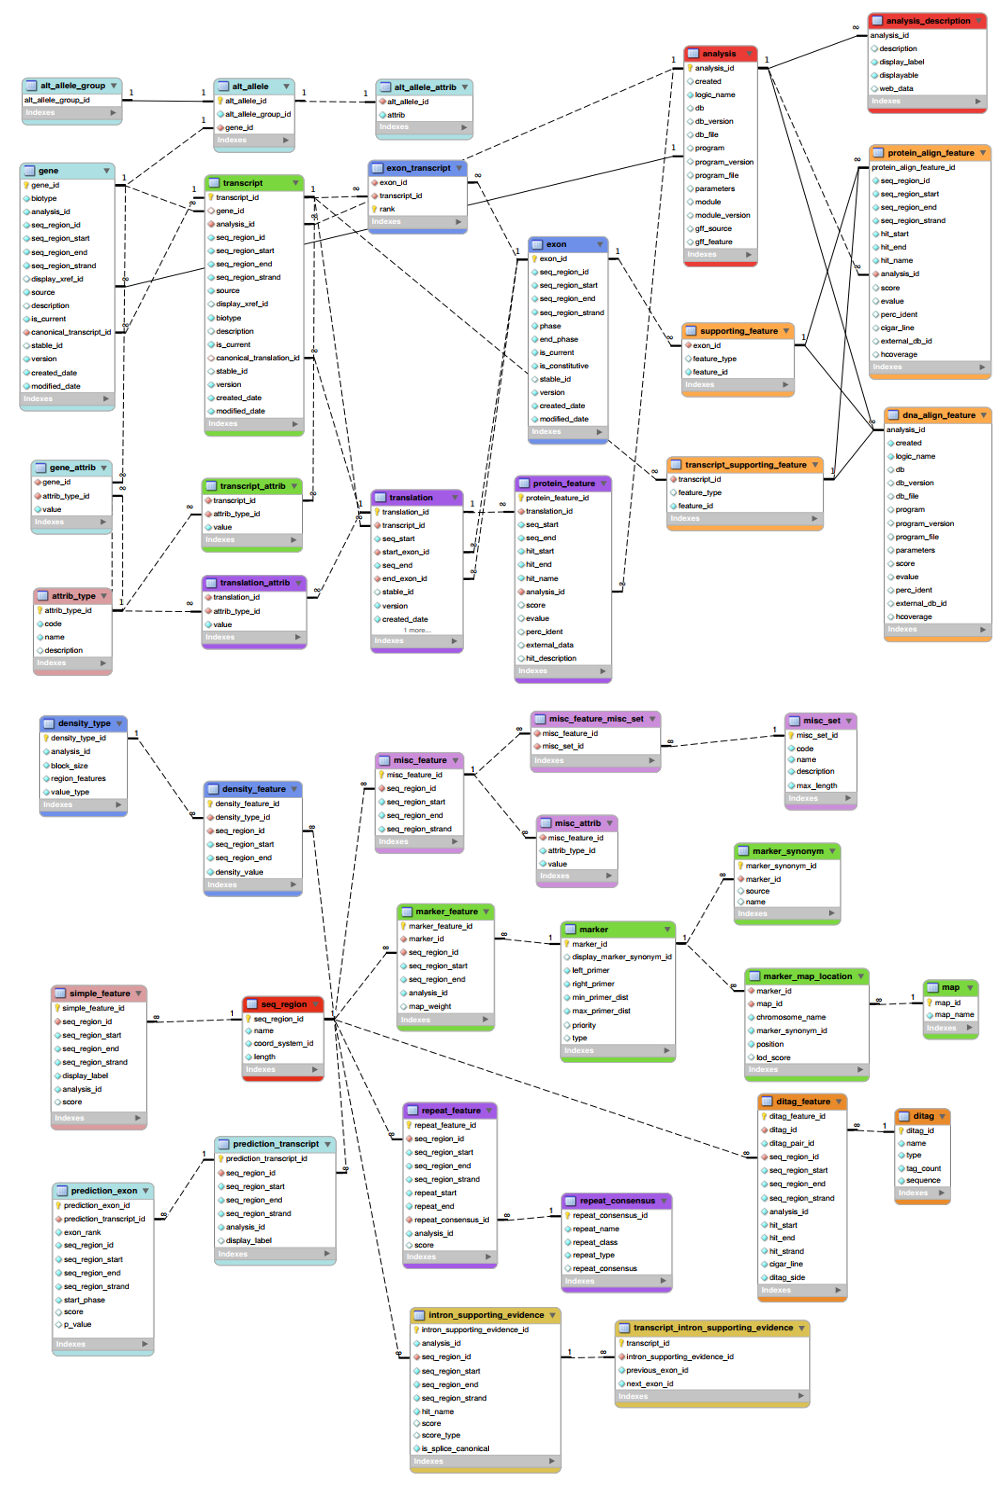
\includegraphics[width=1\textwidth]{img/db-ensembl.png}
		\caption{Fragment schematu bazdy danych EMSEMBL.}
		\vspace{-0.5cm}
		\caption*{\scriptsize Źródło: \url{https://www.ensembl.org/info/docs/api/core/core\_schema.html}}
		\label{img:db-ensebl}
	\end{figure}
		
%%%%%%%%%%%%%%%
	\item \href{http://bioviz.org/igb/index.html}{\emph{IGB}} \label{IGB}
	(rys.\ref{img:przegladarka-igb})
	% https://en.wikipedia.org/wiki/Integrated_Genome_Browser
	% https://bitbucket.org/lorainelab/genoviz-sdk/src
	% https://sourceforge.net/projects/genoviz/
	
	%Integrated Genome Browser to projekt rozpoczęty przez firmę \emph{Affymetrix}, jednak porzucony przez nią i~rozwijany w~środowisku akademickim. Przeglądarka napisana w~Javie, obecnie na prawach Academic free license.
	
	Integrated Genome Browser to projekt używany przez wiele uniwersytetów na całym świecie. Zapoczątkowany przez \emph{Affymetrix}, jednak od 2004 roku jego kod został upubliczniony. Ostatnie wiadomości\footnote{\url{http://bioviz.org/igb/news.html}} odnośnie rozwoju projektu publikowane były w połowie 2016 roku. Oparty na platformie \textit{GenoViz}\footnote{\url{https://sourceforge.net/projects/genoviz/}} dostarczającej re-używalnych komponentów do wizualizacji danych genetycznych. Rozwój platformy zatrzymał się na początku 2016 roku (stwierdzono na podstawie ostatnich commitów\footnote{\url{https://bitbucket.org/lorainelab/genoviz-sdk/commits/all}}) Przeglądarka jest bardzo funkcjonalna - pozwala m.in. na: interaktywną prezentację danych użytkownika akceptowanych w wielu formatach, tworzenie map cieplnych, korzystanie z genomów publicznie dostępnych, wyszukiwanie podobieństw algorytmem BLAST, tworzenie i eksportowanie własnych widoków, udostępnianie danych między współpracownikami, integrację z usługami przechowywania danych, tworzenie własnych pluginów i skryptów.
	\begin{figure}[h]
	% http://bioviz.org/igb/less/images/SlicedView.png
		\centering
		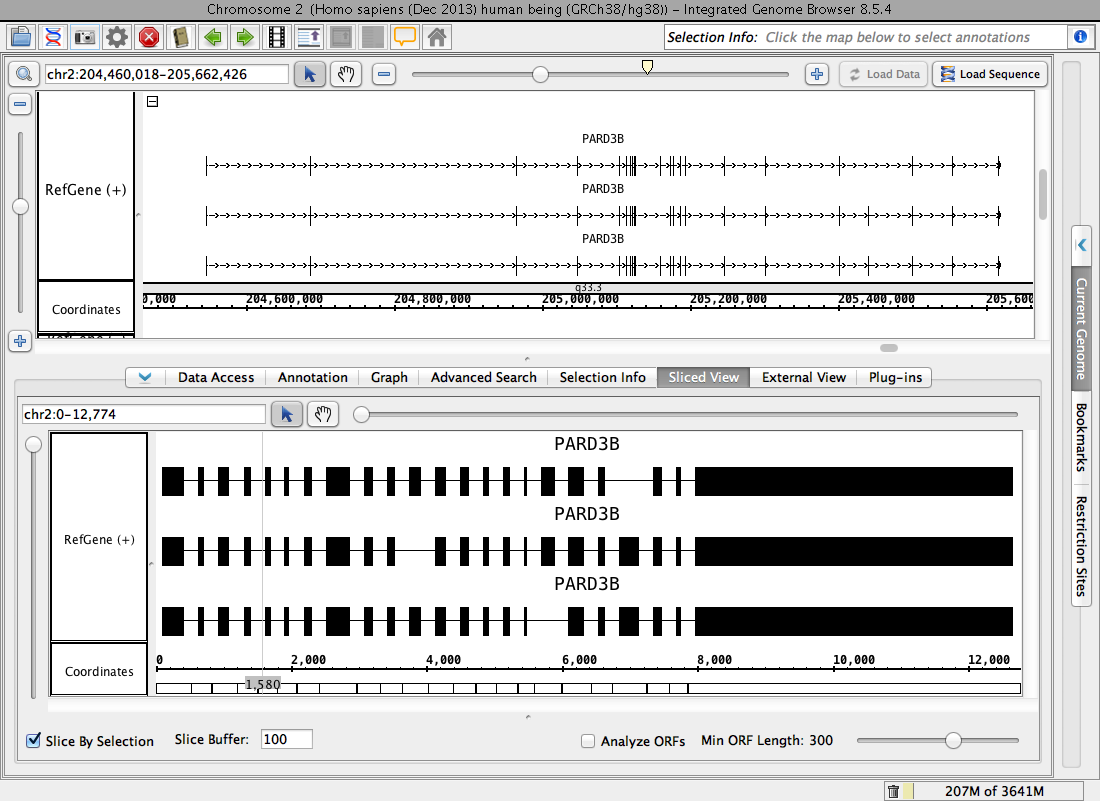
\includegraphics[width=1\textwidth]{img/browser-igb.png}
		\caption{Przeglądarka IGB.}
		\vspace{-0.5cm}
		\caption*{\scriptsize Źródło: \url{http://bioviz.org/igb/less/images/SlicedView.png}}
		\label{img:przegladarka-igb}
	\end{figure}
	
\subsection*{Inne narzędzia}	
	\item \emph{Alamut} \label{alamut} \\
	%http://www.interactive-biosoftware.com/
	przeglądarka oferująca jedynie ludzki genom;
	projekt zamknięty, rozwijany komercyjnie przez firmę \textit{Interactive Biosoftware}; 
	ostatnie wiadomości odnośnie rozwoju projektu z początku 2016 roku\footnote{\url{http://www.interactive-biosoftware.com/media-center/news/}}
	
	\item \emph{Argo Genome Browser} \label{argo-genome-browser} \\
	%http://www.broadinstitute.org/annotation/argo/
	opracowana na \textit{MIT} w \textit{Broad Institute}, który został powołany do życia w 2004 roku. 
	Przeglądarka napisana w języku \textit{Java 1.4}, aktualnie niewspierana - ostatnia wersja wydana na początku 2010 roku. Brak algorytmów KMP, Smitha-Watermana.
	
	\item \emph{ChIPMonk}\\
	%http://www.bioinformatics.babraham.ac.uk/projects/chipmonk/
	projekt opracowany przez \textit{Babraham Bioinformatics} na Uniwersytecie Cambridge, napisany w języku Java, ostatnie wydanie w 2011 roku, oficjalnie przestał być rozwijany.
		
	\item \emph{Biodalliance}\\
	%http://www.biodalliance.org/
	przeglądarka podobna do Ensembl, UCSC czy GBrowse. 
	Wyróżnia się implementacją w nowoczesnych webowych standardach (\textit{HTML5}), uruchamiana w środowisku przeglądarki internetowej. 
	Aktywnie rozwijana, nie wymaga części serwerowej do użytkowania. 
	Brak narzędzi do przeszukiwania genomu w celu znalezienia podobnych sekwencji.
	
	\item \href{https://www.dnanexus.com/genomes/hg18/public_browse}{\emph{DNAnexus}} \label{dnanexus} - przeglądarka do wizualizacji danych korzysta z~technologii \emph{Flash}. Jest narzędziem nowej generacji, mocno rozbudowanym w~kategorii analizy i~obrazowania sekwencji.
	
	\item \href{http://download.cnet.com/GeneWall-Genome-Browser-Pro/3000-2129_4-75855506.html}{\emph{GeneWall}} \label{genewall} - przeglądarka genomów przeznaczona na urządzenia mobilne. W~wersji podstawowej można przeglądać jedynie genom człowieka, natomiast w~wariancie profesjonalnym aplikacji mamy możliwość uploadu własnych plików z~danymi.
	
	\item \href{http://gaggle.systemsbiology.net/docs/geese/genomebrowser/}{\emph{Gaggle Genome Browser}} \label{gaggle} - otwarte narzędzie do mapowania mocno skondensowanych danych na współrzędne genomu. Oprogramowanie przeznaczone do obsługi dużych zbiorów danych, pozwala na łatwy import plików użytkownika. Współpracuje z~innymi bioinformatycznymi narzędziami zawartymi w~frameworku Gaggle.
	
	\item \href{https://genestack.com/}{\emph{Genestack}} \label{genestack} - internetowy, genomiczny system operacyjny. Pozwala wyszukiwać i~importować dane z~wielu publicznych baz danych. Potrafi konwertować dane wejściowe użytkowników z~wielu formatów. Udostępnia zestaw narzędzi dla programistów, do łatwego tworzenia własnych przeglądarek.
	
	\item \href{http://genomeview.org/}{\emph{GenomeView}} \label{genomeview} - samodzielna przeglądarka i~edytor genomu nowej generacji. Obecnie rozwijana przez społeczność \href{http://www.broadinstitute.org/}{Broad Insitute}. Zapewnia interaktywną wizualizację sekwencji, adnotacji, możliwość porównań na wielu poziomach, mapowań i~wielu innych. Dzięki systemowi wtyczek, istnieje możliwość rozszerzenia funkcjonalności przeglądarki.
	
	\item \href{http://www.genomemaps.org/}{\emph{GenomeMaps}} \label{genomemaps} - wysokowydajna przeglądarka z~interfejsem opartym o~HTML5 i~CSS3. W~dużej mierze implementowana z~użyciem biblioteki Javascript \href{https://github.com/opencb/jsorolla}{\mbox{\emph{JSorolla}}}. Dane pozyskuje korzystając z~usług REST bazy \href{https://github.com/opencb/cellbase/wiki}{\emph{CellBase}}. Uruchamia się we wszystkich nowszych przeglądarkach internetowych, nie wymagając od użytkownika instalacji dodatkowych komponentów.
	
	\item \href{http://www.popsci.com/science/article/2011-06/introducing-genome-wowser-ipad-app-lets-you-browse-human-genome}{\emph{Genome Wowser}} - aplikacja przeznaczona na urządzenia mobilne iPad, wydana przez CBMI (ang. Center for Biomedical Informatics) w~Szpitalu Dziecięcym w~Filadelfii. Pozwala przeglądać popularną bazę \emph{UCSC Genome Browser}.
	
	\item \href{https://hyperbrowser.uio.no/hb/}{\emph{Genomic HyperBrowser}} - jest wolnym oprogramowaniem na licencji \emph{GNU GPL v3}. Produkt skupiony głownie na analizie statystycznej elementów w~genomie. Tworzony z~wykorzystaniem platformy \href{https://en.wikipedia.org/wiki/Galaxy_(computational_biology)}{\emph{Galaxy}}.
	
	\item \href{http://wtsi-web.github.io/Genoverse/}{\emph{Genoverse}} - przenośna, konfigurowalna, przeglądarka oparta o~Javasript i~HTML5. Pozwala na eksplorację danych w~dynamiczny, interaktywny sposób. Dane są prezentowane w~przeglądarce, dzięki czemu może być łatwo instalowana na własnych stronach i~pokazywać dane z~wielu źródeł - gromadzonych online i~lokalnie.
	
	\item \href{http://genplay.einstein.yu.edu/}{\emph{GenPlay}} - szybkie i~łatwe w~użyciu narzędzie do analizy i~przetwarzania sekwencji napisane w~Javie. Uruchamia się na większości najpopularniejszych systemów operacyjnych. Prace nad projektem rozpoczęto na Kolegium Medycznym Alberta Einstein'a Uniwersytetu Yeshiva w~Nowym Yorku. Przeglądarka aktualnie w~fazie testowania, używana przez studentów.
	
	\item \href{http://img.jgi.doe.gov/}{\emph{Integrated Microbial Genomes}} - zaawansowany system wspierający analizę i~adnotacje mikrobiologicznych zbiorów danych i~metadanych genetycznych zgromadzonych w~\emph{DOE's Joint Genome Institute}. Współpracuje z~wieloma instytucjami.
	
	\item \href{http://mgv2.cmbi.ru.nl/}{\emph{Microbial Genomic Viewer}} - łatwe w~obsłudze narzędzie do interaktywnej wizualizacji wyników analizy porównawczej genomów. 
	
	\item \href{https://www.nextbio.com}{\emph{NextBio Genome Browser}} - interaktywna aplikacja pozwalająca na wizualizację zależności pomiędzy prywatnymi lub publicznymi zbiorami danych biologicznych różnych typów.
	
	\item \href{http://persephone.net/}{\emph{Persephone}} - rozbudowana aplikacja nowej generacji szeroko używana przez bioinformatyków i~genetyków. Możliwość bezpłatnego korzystania z~wersji \emph{trial} przez 30 dni.
	
	\item \href{http://www.plantgdb.org/}{\emph{PlantGDB}} - przeglądarka z~zestawem narzędzi analitycznych wraz ze zbiorami danych genetycznych wielu roślin.
	
	\item \href{http://tabit.ucsd.edu/}{\emph{STAR}} - zintegrowane środowisko do zarządzania i~wizualizacji danych sekwencjonowania. Płynność działania aplikacji w~przeglądarce internetowej zapewnia połączenie technologi JavaScript, HTML5 i~asynchronicznej komunikacji do wymiany danych. 
	
	\item \href{http://tgac-browser.tgac.ac.uk/}{\emph{TGAC Browser}} - nowa open-source'owa przeglądarka genomów obrazująca adnotacje z~bazy danych \emph{Ensembl}. Wyprodukowana przez \emph{Centrum Analizy Genomów} w~Wielkiej Brytanii (ang.\emph{The Genome Analysis Centre, UK}).
	
	\item \href{http://ugene.net/}{\emph{Ugene}} - darmowa platforma bioinformatyczna wspomagająca użytkowników w~pracach nad sekwencjami. Oferuje narzędzia do analizy danych, przypisów, porównań itp. Dane wejściowe mogą być składowane lokalnie albo udostępnione z~innych źródeł. Napisana w~C++ z~wykorzystaniem biblioteki Qt. Funkcjonuje na licencji GPL.
	
	\item \href{http://enhancer.lbl.gov/}{\emph{VISTA Enhancer Browser}} - kompleksowy zestaw baz danych, narzędzi, serwerów na potrzeby analizy porównawczej sekwencji genomów. Istnieją 2 sposoby na korzystanie z~przeglądarki: można wysyłać własne sekwencje i~dopasowania do analizy, bądź sprawdzać z~wstępnie przetworzonymi danymi całych genomów różnych gatunków. Projekt rozwijany we współpracy z~wieloma instytucjami.
	
	
\end{itemize}